%
%Не забыть:
%--------------------------------------
%Вставить колонтитулы, поменять название на титульнике



%--------------------------------------

\documentclass[a4paper, 12pt]{article} 

%--------------------------------------
%Russian-specific packages
%--------------------------------------
%\usepackage[warn]{mathtext}
\usepackage[T2A]{fontenc}
\usepackage[utf8]{inputenc}
\usepackage[english,russian]{babel}
\usepackage[intlimits]{amsmath}
\usepackage{esint}
%--------------------------------------
%Hyphenation rules
%--------------------------------------
\usepackage{hyphenat}
\hyphenation{ма-те-ма-ти-ка вос-ста-нав-ли-вать}
%--------------------------------------
%Packages
%--------------------------------------
\usepackage{amsmath}
\usepackage{amssymb}
\usepackage{amsfonts}
\usepackage{amsthm}
\usepackage{latexsym}
\usepackage{mathtools}
\usepackage{etoolbox}%Булевые операторы
\usepackage{extsizes}%Выставление произвольного шрифта в \documentclass
\usepackage{geometry}%Разметка листа
\usepackage{indentfirst}
\usepackage{wrapfig}%Создание обтекаемых текстом объектов
\usepackage{fancyhdr}%Создание колонтитулов
\usepackage{setspace}%Настройка интерлиньяжа
\usepackage{lastpage}%Вывод номера последней страницы в документе, \lastpage
\usepackage{soul}%Изменение параметров начертания
\usepackage{hyperref}%Две строчки с настройкой гиперссылок внутри получаеммого
\usepackage[usenames,dvipsnames,svgnames,table,rgb]{xcolor}% pdf-документа
\usepackage{multicol}%Позволяет писать текст в несколько колонок
\usepackage{cite}%Работа с библиографией
\usepackage{subfigure}% Человеческая вставка нескольких картинок
\usepackage{tikz}%Рисование рисунков
\usepackage{float}% Возможность ставить H в положениях картинки
% Для картинок Моти
\usepackage{misccorr}
\usepackage{lscape}
\usepackage{cmap}



\usepackage{graphicx,xcolor}
\graphicspath{{Pictures/}}
\DeclareGraphicsExtensions{.pdf,.png,.jpg}

%----------------------------------------
%Список окружений
%----------------------------------------
\newenvironment {theor}[2]
{\smallskip \par \textbf{#1.} \textit{#2}  \par $\blacktriangleleft$}
{\flushright{$\blacktriangleright$} \medskip \par} %лемма/теорема с доказательством
\newenvironment {proofn}
{\par $\blacktriangleleft$}
{$\blacktriangleright$ \par} %доказательство
%----------------------------------------
%Список команд
%----------------------------------------
\newcommand{\grad}
{\mathop{\mathrm{grad}}\nolimits\,} %градиент

\newcommand{\diver}
{\mathop{\mathrm{div}}\nolimits\,} %дивергенция

\newcommand{\rot}
{\ensuremath{\mathrm{rot}}\,}

\newcommand{\Def}[1]
{\underline{\textbf{#1}}} %определение

\newcommand{\RN}[1]
{\MakeUppercase{\romannumeral #1}} %римские цифры

\newcommand {\theornp}[2]
{\textbf{#1.} \textit{ #2} \par} %Написание леммы/теоремы без доказательства

\newcommand{\qrq}
{\ensuremath{\quad \Rightarrow \quad}} %Человеческий знак следствия

\newcommand{\const}{\text{const}} % Написание const в формулах

\newcommand{\qlrq}
{\ensuremath{\quad \Leftrightarrow \quad}} %Человеческий знак равносильности

\renewcommand{\phi}{\varphi} %Нормальный знак фи

\newcommand{\me}
{\ensuremath{\mathbb{E}}}

\newcommand{\md}
{\ensuremath{\mathbb{D}}}



%\renewcommand{\vec}{\overline}




%----------------------------------------
%Разметка листа
%----------------------------------------
\geometry{top = 3cm}
\geometry{bottom = 2cm}
\geometry{left = 1.5cm}
\geometry{right = 1.5cm}
%----------------------------------------
%Колонтитулы
%----------------------------------------
\pagestyle{fancy}%Создание колонтитулов
\fancyhead{}
%\fancyfoot{}
\fancyhead[R]{\textsc{Экзамен. Оптика}}%Вставить колонтитул сюда
%----------------------------------------
%Интерлиньяж (расстояния между строчками)
%----------------------------------------
%\onehalfspacing -- интерлиньяж 1.5
%\doublespacing -- интерлиньяж 2
%----------------------------------------
%Настройка гиперссылок
%----------------------------------------
\hypersetup{				% Гиперссылки
	unicode=true,           % русские буквы в раздела PDF
	pdftitle={Заголовок},   % Заголовок
	pdfauthor={Автор},      % Автор
	pdfsubject={Тема},      % Тема
	pdfcreator={Создатель}, % Создатель
	pdfproducer={Производитель}, % Производитель
	pdfkeywords={keyword1} {key2} {key3}, % Ключевые слова
	colorlinks=true,       	% false: ссылки в рамках; true: цветные ссылки
	linkcolor=blue,          % внутренние ссылки
	citecolor=blue,        % на библиографию
	filecolor=magenta,      % на файлы
	urlcolor=cyan           % на URL
}
%----------------------------------------
%Работа с библиографией (как бич)
%----------------------------------------
\renewcommand{\refname}{Список литературы}%Изменение названия списка литературы для article
%\renewcommand{\bibname}{Список литературы}%Изменение названия списка литературы для book и report
%----------------------------------------

\begin{document}
	\section{Явление полного внутреннего отражения, его применения. Оптические элементы и
		приборы, работающие на явлении полного внутреннего отражения. Оптоволокно,
		типы оптоволокна.}
	Сначала наивное. Мы знаем формулу Снеллиуса $\sin \theta = n_{21} \sin \theta'$, где $n_{21}$ -- это относительная оптическая плотность. Если $n_{21} < 1$ то должен существовать такой угол падения $\arcsin n_{21}$ после которого не может уже существовать никакого прошедшего луча, а только отраженный. Так как свету некуда деться, кроме как отразиться, то он отражается полностью. 
	
	Теперь как это выглядит с точки зрения волновой оптики (Сивухин с 402)\\
	Пусть у нас есть падающая волна:
	\begin{align*}
		E^{e} = \mathcal{E} e^{i(\omega t - k_1 r)}
	\end{align*}
	Мы из соображений геометрической оптики знаем, что должны быть еще отраженная (r) и прошедшая (d) волны:
	\begin{align*}
	E^{r} = \mathcal{R} e^{i(\omega t - k'_1 r)}\\E^{d} = \mathcal{D} e^{i(\omega t - k_2 r)}
	\end{align*}
	Мы предполагаем что они тоже плоские из соображений симметрии. Равенство частот у всех трех объясняется тем, что напряженности могут иметь только гармоническую зависимость от времени, а в случае наложения двух плоских полей с разными частотами такое не выполняется.\\
	Из соотношений симметрии надо заключить, что касательная к плоскости составляющая волнового вектора у всех трех волн одинаковая. В нашем случае это проекция на ось x (смотри рисунок)
	\begin{figure}[H]
		\includegraphics*[scale = 0.3]{2_1}
	\end{figure}
	То есть: $k_{1x} = k'_{1x} = k_{2x}$\\
	Так же можем написать про волновые вектора:
	\begin{align*}
	k_1^2 = k_1'^2 = \dfrac{\omega^2 }{c^2 } \varepsilon_1\\
	k_2^2 = \dfrac{\omega^2 }{c^2 } \varepsilon_2
	\end{align*}
	Где эпсилон 1 и 2 это диэлектрическая проницаемость среды из которой пришел луч и в которую ушел соответственно. Отсюда можно узнать их z составляющие:
	\begin{align*}
	k'_{1z} = - \sqrt{k_1^2 - k_{1x}^2}\\
	k_{2z} = \sqrt{k_2^2 - k_{1x}^2}	
	\end{align*}
	Так как нас волнует полное внутреннее отражение, то рассмотрим случай, когда $k_2^2 < k_{1x}^2 $ так как $k_{1x} = k_1 \sin \phi$, то это условие равносильно условию $\sin \phi > \sqrt{\dfrac{\varepsilon_2}{\varepsilon_1}} = n_{21}$ так же как в геометрической оптике. Естественно чтобы такое условие вообще могло выполняться надо чтобы $n_{21}<1$. В этом случае $k_{2z}$ комплексный. Обозначим так: $k_{2z} = \dfrac{-i}{2h}$ Почему минус? Потому что корень это функция многозначная и нужную ветвь мы выбираем исходя из физических требований, а тут нужен как раз минус. Со всем этим можем написать отраженную волну как:
	\begin{align*}
	E^{d} = \mathcal{D}e^{-z/2h} e^{i(\omega t - k_{1x} x)}\\
	h = \dfrac{\lambda_1}{4\pi \sqrt{\sin^2 \phi  - n_{21}^2}}
	\end{align*}
	То есть волна идет вдоль границы, но затухает вглубь вещества (см рисунок)
	\begin{figure}[H]
		\centering
		\caption{Опыт Мандельштама и Селени}
		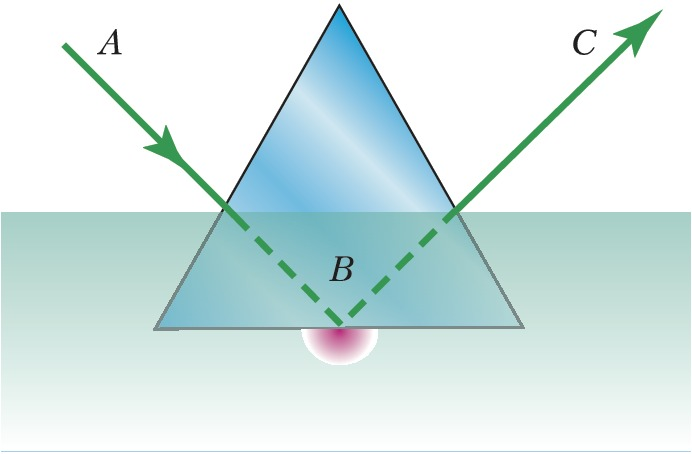
\includegraphics[scale = 1]{2_2}
	
	\end{figure}
	Эффект полного внутреннего отражения используется например в уголковых отражателях и во многих других призмах:
		\begin{figure}[H]
			\centering
			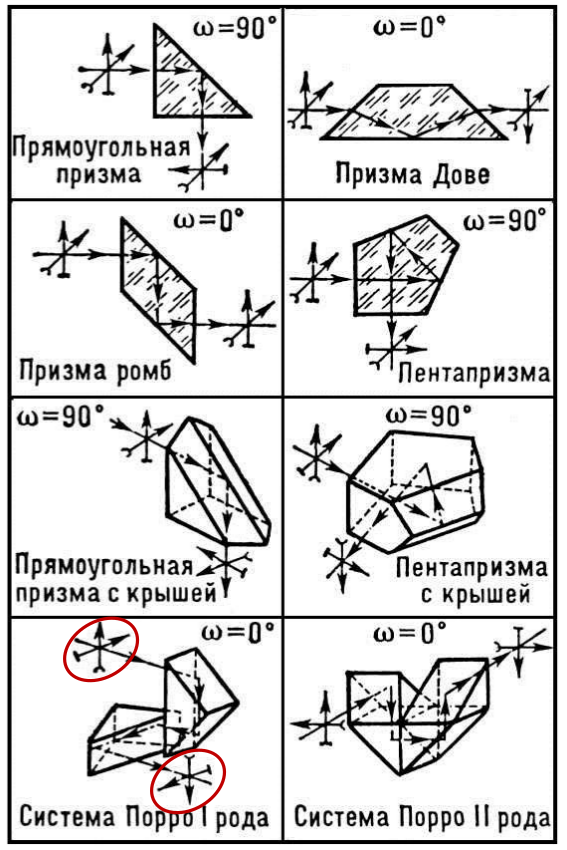
\includegraphics[scale = 0.3]{2_3}
		\end{figure}
	Оптоволокно это такая штука, в которой свет постоянно испытывает отражения от стенок. Состоит из двух слоев очевидно. Внешний имеет оптическую плотность больше. Заодно он защищает внутренний слой от повреждений. Сгибать сильно нельзя.
\end{document}